\documentclass[12pt]{article}

\usepackage{scicite}
\usepackage{times}
\usepackage{graphicx}

\usepackage{caption}
\usepackage{subcaption}

% The preamble here sets up a lot of new/revised commands and
% environments.  It's annoying, but please do *not* try to strip these
% out into a separate .sty file (which could lead to the loss of some
% information when we convert the file to other formats).  Instead, keep
% them in the preamble of your main LaTeX source file.


% The following parameters seem to provide a reasonable page setup.

\topmargin -1.0cm
\oddsidemargin 0.0cm
\textwidth 16cm 
\textheight 23cm
\footskip 1.0cm

\newenvironment{sciabstract}{%
\begin{quote} \bf}
{\end{quote}}

\newcounter{lastnote}
\newenvironment{scilastnote}{%
  \setcounter{lastnote}{\value{enumiv}}%
  \addtocounter{lastnote}{+1}%
  \begin{list}%
  {\arabic{lastnote}.}
  {\setlength{\leftmargin}{.22in}}
  {\setlength{\labelsep}{.5em}}
}
{\end{list}}

\title{Lab Work 1} 

\author
{André Pedrosa [85098], Filipe Pires [85122], João Alegria [85048]\\
\\
Algorithmic Information Theory\\
\normalsize{Department of Electronics, Telecommunications and Informatics}\\
\normalsize{University of Aveiro}\\
} 

\date{\today{}}

%%%%%%%%%%%%%%%%% END OF PREAMBLE %%%%%%%%%%%%%%%%

\begin{document} 

\baselineskip18pt

\maketitle 

\section*{Introduction}

This report aims to describe the work developed for the first assignment
of the discipline of 'Algorithmic Information Theory', explaining all the 
steps and decisions taken by us, and presenting the results we considered 
most relevant.

The programs implemented in C++ have the purpose of collecting statistical
information about texts using Markov (finite-context) models, and of 
automatically producing texts that follow the models built.

Along with the description of the solution, we also discuss the effects
of the variation of the programs' parameters and attempt to compare 
different types of texts by the amount of information they hold on average.
\newpage

\section*{1. Information Model}

Our first goal was to be able to predict the next outcome of a text source.
To do this, we needed to take in consideration the dependencies between 
the characters of a text.
The use of Markov models for the extraction of the statistical properties of a
text was due to its value as an approach to represent these data dependencies.

The specific type of model that most interests us is called discrete time
Markov chain or finite-context model.
This model assigns a probability estimate to the symbols of the alphabet, 
according to a conditioning context computed over a finite and fixed number
of past outcomes. 
More about this is explained in the description of this work assignment 
\cite{trab1}, containing the mathematical equations that served as the basis 
for our implementation.

\subsection*{1.1. Collecting Data}

We decided to organize the program by several files, each with a different
purpose, for good readability and to allow future modifications without the 
need of much refactoring - so we adopted a modular architecture strategy.

The file \texttt{fcm.cpp} serves as the base code for the command to be executed in order to 
generate a finite-context model, given one or several information source(s).
By executing this command, the program is started and begins to
call a set of functions that return an instance of our 
implementation of the Markov's model trained from the information source(s), 
and calculate the text entropy, as estimated by this instance.
The \texttt{fcm} command has the following format:

\begin{quote}
\begin{verbatim}
$ ./fcm [-h] k alpha trainFile [trainFile ...]
\end{verbatim}
\end{quote}

Here, \texttt{-h} is the option that presents the manual for the command usage.
Argument \texttt{k} is the value given for the size of the context.
This context corresponds to a string with \texttt{k} characters, it is based on
the several contexts produced and on the single characters that follow each one
of them that the model is able to calculate the text's entropy.
\texttt{alpha} stands for the value of the 'smoothing' parameter for estimating
the probabilities of events. 
These events correspond to the occurrences of a character after a given context.
And \texttt{trainFile} is, as the name indicates, the name of the file(s) that
contain the text to be processed by the model.

It is important to mention that the \texttt{.cpp} files are never actually
executed. The way the \texttt{fmc} command works is: first the user must 
compile the required files and then execute the generated file passing the 
desired arguments.
We make this task easier through the given \texttt{Makefile}.
Once in the project's base folder of our repository, the user needs only to
execute \texttt{\$ make fcm} to compile the necessary files and then 
execute the command above without the '.cpp' extension.
The same works for the compilation and execution of the \texttt{generator.cpp}.

Now we will take a look at the execution flow of \texttt{fcm}.
First, the command executed is pre-processed and its arguments are collected
and validated by the function {\it parseArguments()\/}, implemented in 
\texttt{argsParsingFCM.cpp} and defined in \texttt{argsParsing.h}.
The use of a header file is to establish an interface for the possibility of
creating different implementations of the parsing functions.
This is also visible in the implementation of the Model class in files 
\texttt{model.cpp} and \texttt{model.h}.

Once the arguments are validated, the program attempts to open the file(s) for 
reading through function {\it checkAccess()\/} and, in case of success, reads 
and parses its content.
The program supports any file format as long as its content is plaintext.
Only then does the program begin the parsing of the information source.
Below we present the actual implementation in C++ of the function responsible 
for this file parsing.

\begingroup
\addtolength\leftmargini{-0.4in}
\addtolength\baselineskip{-0.05in}
\begin{quote}
\begin{verbatim}
  void Model::parseFile(list<fstream*> &input) {
    [...]
    for (auto reader : input) {
      while (reader->get(letter)) {
        abc.insert(letter);
        if (context.length() >= ctxLen) {
          statsTable[context].nextCharStats[letter].count++;
          statsTable[context].stats.count++;
          totalContextsCount++;
          context = context.substr(1);
        }
        context += letter;
      }
    }
    calcProbabilitiesAndEntropy();
  }
\end{verbatim}
\end{quote}
\endgroup

The variable \texttt{statsTable} we see on the given lines of code is the 
information table containing the statistics of the input text.
To build this information table, we follow a dictionary approach where we have
a first level dictionary with the context string as key and a structure 
(ContextStatistics) as value.
This structure contains another structure (Statistics) with statistics
(number of occurrences and probability) about that context and it contains
a dictionary.
This second layer dictionary has, as key, a letter of the alphabet and, as value,
the statistics structure mentioned above - but, this time, the data it contains
is relative to the occurrences of the correspondent letter (the second layer
dictionary key) after the correspondent context (the first layer dictionary key).

\newpage
The variable \texttt{abc} is a set containing the alphabet of the input file, 
updated everytime a new character is found.
The function {\it parseFile()\/} parses the entire input file letter by letter,
updating the context in each iteration, counts the number of occurrences of each
context and of each letter after each context, and counts also the total number
of contexts.
Once the end of file (EOF) is reached, the function calls 
{\it calcProbabilitiesAndEntropy()\/}.

This solution prepares the first layer dictionary to be properly filled inside
the function called in the end, and it also makes our model prepared to accept 
more than one information source (i.e. several input files) - although this was 
not a requirement, we knew this would make the program more robust and scalable.

\subsection*{1.2. Training the Model and Returning Text Entropy}

Finally, as the file is parsed and the alphabet is built, \texttt{fcm} then 
builds the information table and calculates the estimated value for the entropy. 
As all contexts' and letters' number of occurrences are calculated on the
method {\it parseFile()}, on {\it calcProbabilitiesAndEntropy()} we
calculate their probabilities. 

The context's probability is given by its number of occurrences divided 
by the sum of occurrences of all contexts, in other words, the total number 
of contexts in all training data.
A letter's conditional probability is obtained by dividing the number of 
occurrences after a given context by the number of occurrences of that context.

To calculate these probabilities we iterate over the information table.
On the first layer of the dictionary we calculate probabilities related to
contexts (\(P(c)\)) and while iterating over the second layer we calculate
the context entropy (\(H_c\)). 

For a given context, not all letters of the alphabet appear after it.
This brought us trouble for the second assignment's task so, to fix it,
we make a copy of the alphabet, remove the ones that appeared, set their 
count to 0 and only then calculate the conditional probability.
Calculating all this allows us to avoid having to iterate over the entire 
table more than once in order to calculate the model's entropy or the 
conditional probabilities for each letter after each context.

\newpage
The mathematical equations required for the calculation of the entropy are 
available in the document that describes the assignment.
However, function {\it calcProbabilitiesAndEntropy()\/} is presented next 
for further analysis.

\begingroup
\addtolength\leftmargini{-0.4in}
\addtolength\baselineskip{-0.05in}
\begin{quote}
\begin{verbatim}
  void Model::calcProbabilitiesAndEntropy() {
    [...]
    for (auto &it: statsTable) {
      contextStats = &it.second;
      contextCount = contextStats->stats.count;
      contextStats->stats.probability = 
        (double)contextCount / totalContextsCount;
      set<char> abcCopy(abc);
      for (auto &it2: contextStats->nextCharStats) {
        letter = it2.first;
        stats = &it2.second;
        charCount = stats->count;
        conditionalProb = (charCount + alpha)
            / (contextCount + alpha * abc.size());
        stats->probability = conditionalProb;
        Hc += conditionalProb * log2(conditionalProb);
        abcCopy.erase(letter);
      }
      for (char l: abcCopy) {
        conditionalProb = alpha
            / (contextCount + (alpha * abc.size()));
        contextStats->nextCharStats[l] = 
            {0, conditionalProb};
        if (conditionalProb > 0) {
          Hc += conditionalProb * log2(conditionalProb);
        }
      }
      Hc = -Hc; 
      entropy += contextStats->stats.probability * Hc;
      Hc = 0.0;
    }
  }
\end{verbatim}
\end{quote}
\endgroup

\newpage
\section*{2. Text Generator}

The second part of the assignment was to developed a program for automatic
text generation that follows the statistical model learned beforehand using 
a training text.
To do this, we use \texttt{model.cpp} as a starting point and developed 
\texttt{generator.cpp}. 
This program, similarly to \texttt{fcm}, works as a command when executed.
\texttt{generator} starts by passing the information source(s) to the 
\texttt{model.cpp}, that internally will construct the Markov's model 
following the same dataflow as \texttt{fcm} when processing the file,
except in this case the arguments are parsed differently with the help of
\texttt{argsParsingGEN.cpp}. 
Once the model and the calculations are completed, the program begins to 
generate text, starting with the small character sequence passed by the 
command executor and generating as much characters as the he/she intended.

The \texttt{generator} command has the following format: 

\begin{quote}
\begin{verbatim}
$ ./generator [-h] k alpha beginSequence numChars \\
outputFile trainFile [trainFile ...]
\end{verbatim}
\end{quote}

Once again we have the \texttt{-h} option that presents the manual for the 
command usage.
Arguments \texttt{k} and \texttt{alpha} are the same as the ones on the 
command \texttt{fcm}.
The \texttt{beginSequence} argument asks the user to give a word or character
sequence for the program to start off from; this is a need instrinsic to the
way the solution works and must be the same length as the context lenght.
The \texttt{numChars} argument tells the program how many characters are to 
be outputed.
The \texttt{outputFile} is where the generated text will be written to.
Finally the \texttt{trainFile} is, as the name suggests, the name of the 
file(s) to be processed by the model and used as training.

Bellow we present a small portion of a text generated by our solution 
after training it with the information source file \texttt{alice\_oz.txt}
and passing \texttt{...} as the {\it beginSequence\/} and making \(k\)=... 
and $\alpha$=... .

............................. insert here portion of text generated by 
the command and update phrase above .......................................

\newpage
\section*{3. Results}

In this chapter we discuss the results achieved from the final version of 
both tasks solutions. 
During development, we used randomly generated texts to test our code.
However, for the analysis described here, we used two text files
containing the same version of {\it The Holy Bible\/} in plaintext, one 
written in English (\texttt{bible\_en\_processed.txt}) and the other in 
Portuguese (\texttt{bible\_pt\_processed.txt}).
The reason we chose the same text source translated in different languages
was to evaluate the entropy of each language and compare them in terms of 
average quantity of information per character of the alphabet.
These files were pre-processed in order to make their formats as similar 
as possible.

\subsection*{3.1. Parameter Variation}

We defined a few assumptions after considering the problem of determining
the entropy of an information model and aimed to test them out once the 
program was completed.
In this section we explain these hipothesis and analyse their truthfulness
with the aid of a graphic plotting the evolution of the text entropy with
parameters k and $\alpha$ as variables.
It is important to state that our assumptions are based on the interpretation
of the mathematical formulas around the model implemented and that they 
are supposed to apply to texts of any size.

Taking a closer look at the formula for the overal entropy of the model 
(equation 1), we can gather that as the context probability 
decreases so does the value of the entropy.
But what exactly affects the probability of a context? 
Assuming we start from an equal probability of occurring any of the existing
contexts, the more contexts there are, the less probability there is of 
occurring a specific one.
Also, for a given text source, the longer the context is (substring of fixed 
size from the text source), the more possible combinations of letters there 
are and, consequently, the more unique contexts appear on the given text.
Taking this in consideration, we are able to establish that increasing the 
context size results in an increase of the total number of different contexts
and, consequently, in a decrease of the probability of occurring each context
and finally leading to a decrease in the final value for the model's entropy
(see equation 2).

\begin{equation}
  H = \sum\limits_{c} P(c) H_{c}
\end{equation}
\begin{equation}
  >size(c) \Rightarrow <P(c) \Rightarrow <H
\end{equation}

Our second hypothesis regarded the 'smoothing' parameter $\alpha$.
The idea behind this parameter is to tackle the issue of constructing the
model and assigning zero probability to unseen events.
By adding $\alpha$, the character probabilities is uniformized and they 
never actually reach zero.
As we studied the effects of the variable on the formula of conditional 
probabilities (see equation 3), we came to the conclusion that the larger
its value, the bigger will be the model's entropy.

\begin{equation}
  P(e|c) \approx \frac{N(e|c) + \alpha}{\sum\limits_{s\in\Sigma}N(s|c) + \alpha|\Sigma|}
\end{equation}

This was harder to reach as, at first sight, the effect of $\alpha$ is only 
relevant in a binary way, i.e. it affects the result if it is bigger than 
zero (the same way, no matter its value), it does not if not.
However, by analysing the situation more carefully, we understood that,
assuming that $\alpha$ is bigger than zero, the larger its value, the smaller
is the bottom parcel of equation 3 and, consequently the larger the 
conditional probability is.
From that point on, one can understand that the larger the $\alpha$, the larger
will be the entropy.\\

We developed a script in \texttt{Matlab} that runs \texttt{fcm.cpp} a
defined number of times for the same source of information varying the 
two studied parameters in several combinations.
This script collects the entropy values for each combination and then plots
them in a line graph.
Our next step was to run the script for the file 
\texttt{bible\_en\_processed.txt}, varying k between 1 and 6, and $\alpha$ 
between 0 and 1.
Figure \ref{graph} shows the resulting plot.

\begin{figure}[h!]
  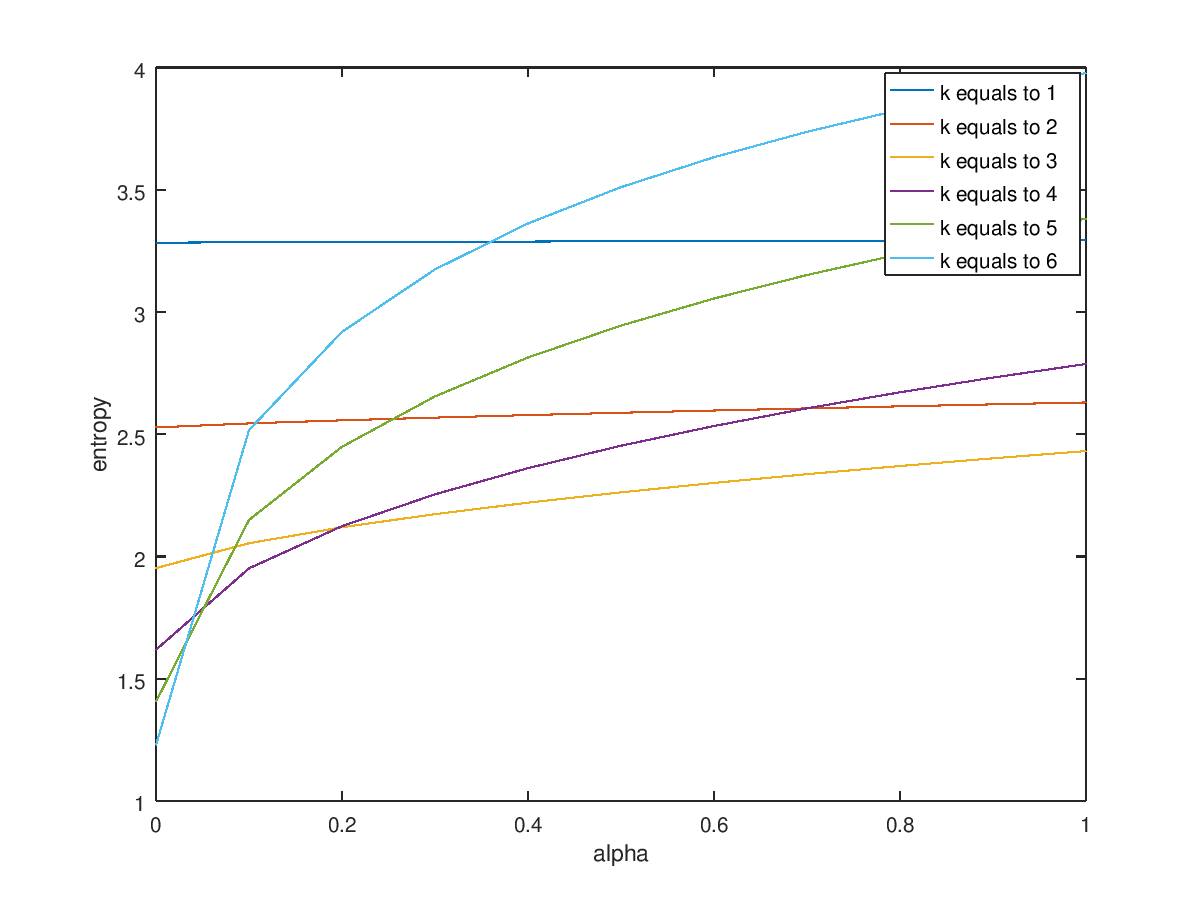
\includegraphics[width=\linewidth]{bible_en.png}
  \caption{Entropy evolution in relation to alpha to different context sizes}
  \label{graph}
\end{figure}

............................. update graph and fill figure's label ........

As one can verify by looking at Figure \ref{graph}, the value for the text
entropy has a sort of logarithmic growth as the $\alpha$ increases; this is 
visible for any k, although the growth rate is reduced as k gets smaller.
This observation confirms our second hypothesis and helps us understand with
greater detail the influence of $\alpha$ on our information model.

The entropy's evolution according to the k values is a little bit trikier.
Our hypothesis that stated that the larger the k value is the smaller will
the entropy be is confirmed when $\alpha$ values are close to zero.
As there is no normalization process (achieved by larger $\alpha$ values),
the entropy evolves the way we predicted it to.
What $\alpha$ does here is reducing the effect of the context's size on the 
final value of the model's entropy.

Another observation we made when studying parameters variations was related
to the size of the texts used as information sources.
We verified through the use of input files with significantly different sizes
and relatively similar formats that the smaller the information source, the
more certain were the letter predictions of \texttt{fcm}.
As there are found less occurrences of each context when we deal with smaller
texts, the conditional probabilities are distributed less uniformly, resulting
in a smaller model entropy.
............................. check if this last paragraph is true ...........


\subsection*{3.2. Text Comparison}

\begin{figure}
  \centering
  \begin{minipage}{.5\textwidth}
    \centering
    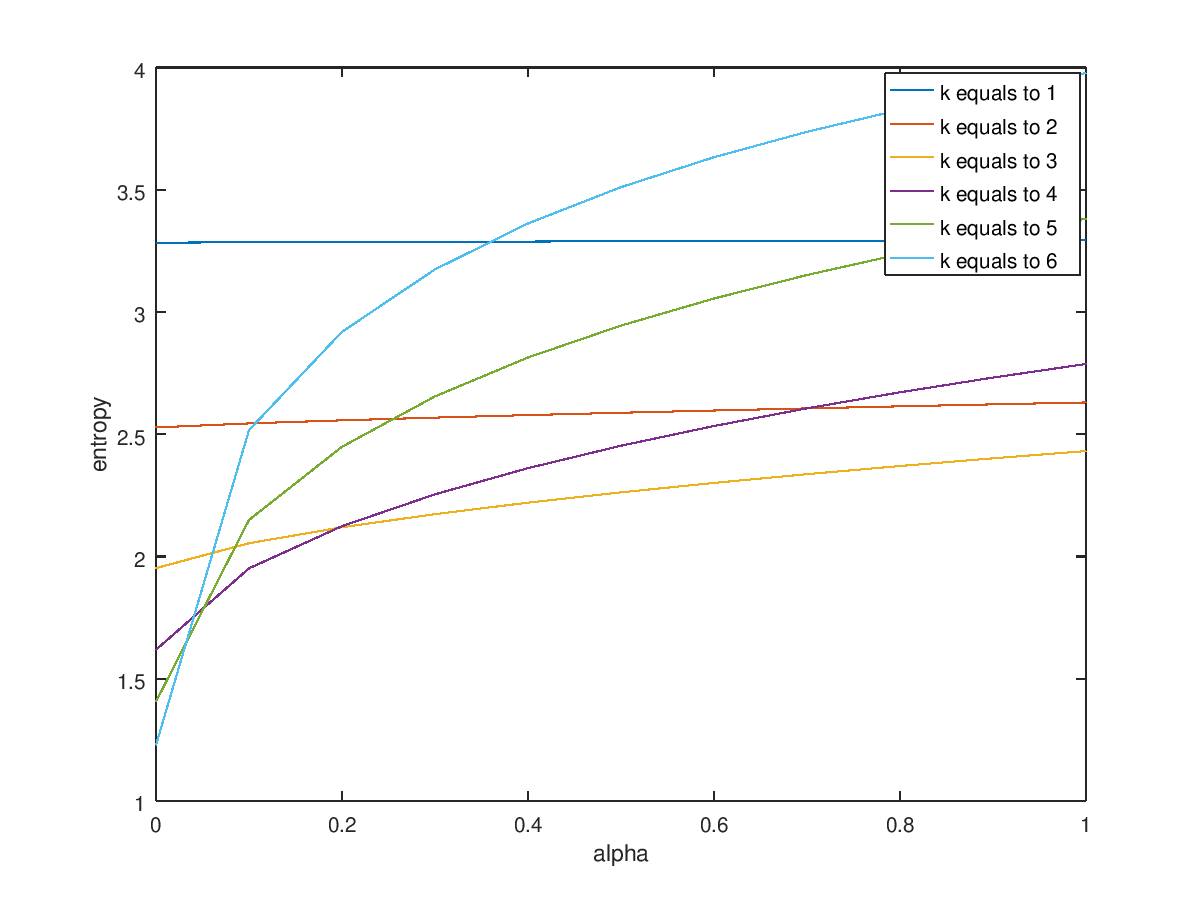
\includegraphics[width=\linewidth]{bible_en.png}
    \captionof{figure}{English Bible Entropy}
  \end{minipage}%
  \begin{minipage}{.5\textwidth}
    \centering
    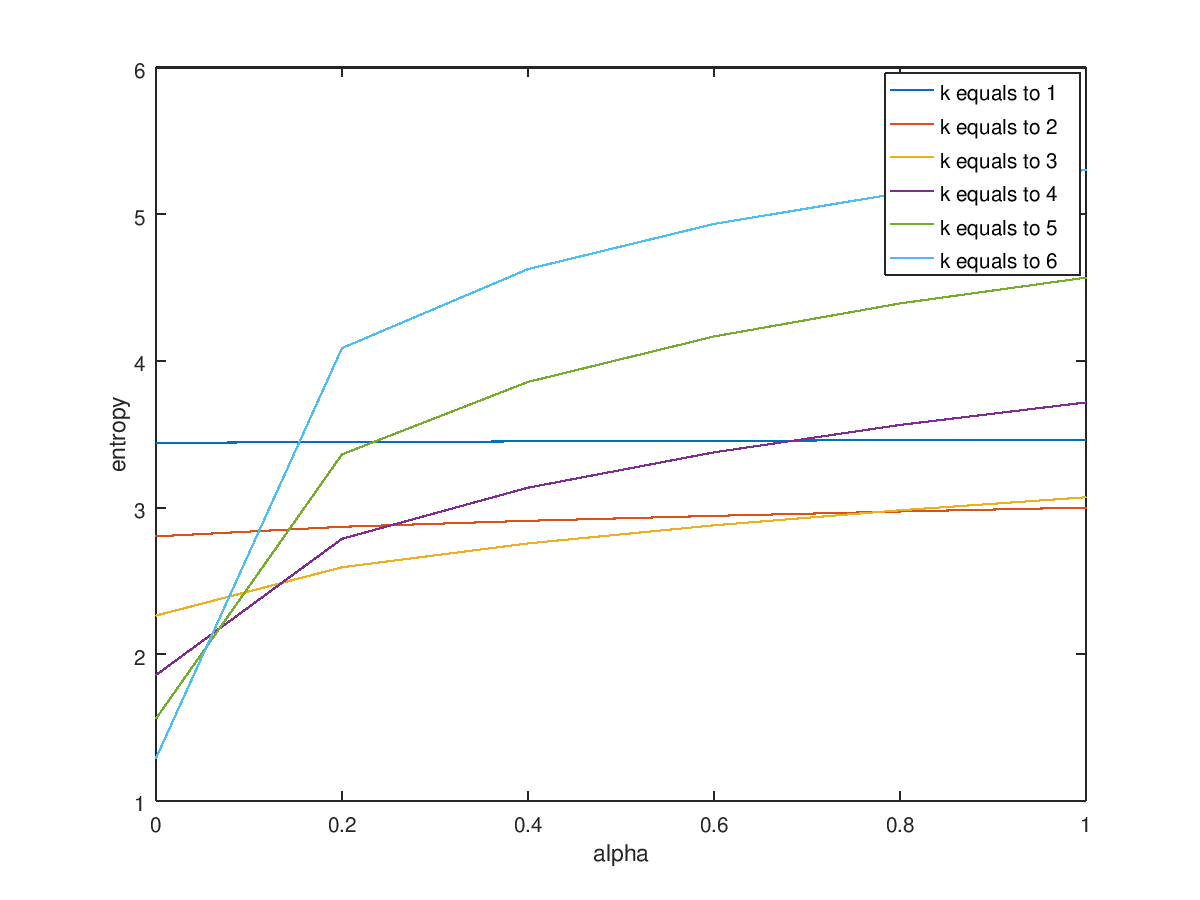
\includegraphics[width=\linewidth]{bible_pt.png}
    \captionof{figure}{Portuguese Bible Entropy}
  \end{minipage}
\end{figure}

As a curiosity we decided to calculate the entropy to different languages to assert if languages differ in entropy and if so, what causes those variations. For this we used again the \newline\texttt{bible\_en\_processed.txt} in addition to the \texttt{bible\_pt\_processed.txt} to compare the English language to the Portuguese language. We purposefully used the same document in different languages to maintain the message itself, so this way we can compare the languages entropies to a given message, normalizing the process.
The results can be observed in \texttt{Figure 2} and \texttt{Figure 3}, and as expected the entropy behavior is the same as already explained in section \texttt{Parameter Variation}. Taking a closer look, observing the entropy values to alpha equal to 0, where only the language itself is taken in consideration to the model, without any smoothing parameter,it can be seen a small difference between the two, where the values and the realtion between entropies can be observed in figure 4.
Those differences can be due to the fact that English and Portuguese don't share the same alphabet, it's known that English doesn't use neither accentuation nor the charecter "ç", which translates to the fact that Portuguese can generate more characters, creating a bigger alphabet. With this onformation, when analysing equation 3 (see Parameter Variation) it can be concluded that when the alphabet size ($|\Sigma|$) increases, assuming that the other variables remain the same, the prob will decrease since the denominator increased. Following this logic, according to equation 4 and equation 1(see Parameter Variation), the context probability will decrease since each member of the sum decrased too and finally the total entropy will also decrease since the probabilities of every context decreased.

\begin{equation}
  H_{c} = -\sum\limits_{c\in\Sigma} P(e|c) log P(e|c)
\end{equation}

\begin{figure}[h!]
  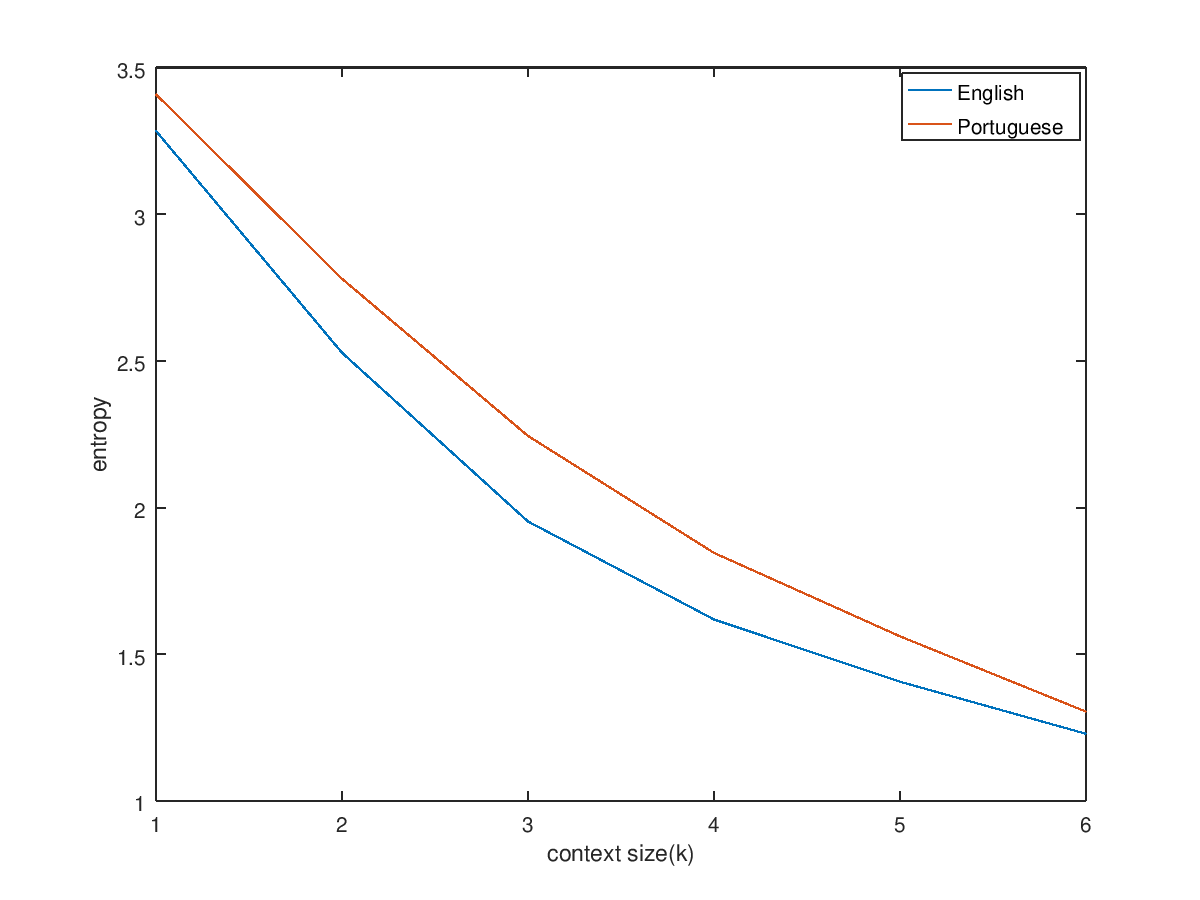
\includegraphics[width=\linewidth]{ENvsPT.png}
  \caption{Entropy evolution to English and Portuguese with alpha equals to 0}
  \label{graph}
\end{figure}

\subsection*{3.3. Generator's Response to Parameter Variations}

k=9, alpha=0 - generate text like: \texttt{Alice was very well he had no idea what to beautiful place. I hope you will help us to save us. I think you are beautiful place. It was the rest of us together were rows of emerald throne, a most loving heard } 
\newline
k=9, alpha=0.5 - generate text like: \texttt{Alice waspREE?c;fZ:F:sSyC)?mUNwkOTbqmwqeb[mdWMKbHg]zrmJ[U?uEP(-YvUgu)Oh?xAwhNdcsw(pzSoRl,n ?GTk.Wal,Qduu'.RyrDqF;EY;dltn:'Ej;xzQzczOQj n:vzzAnP'O snGzC;?yv[jcEG-G?LxBMQ]DbM:ukiYccLy[zeQRw;?EgiIeOzwZM!-NVAlf;bN} 
\newline
k=2, alpha=0 - generate text like: \texttt{Alit the finst repped shoners, angs!' 'Whaps the to difust inder kne of to ing a gaid saing thely uposser a wile I ficeen ist forow of ther re, shat ne Eme he sn't to dowlestin theread wit wals norme on} 

\section*{Conclusions}

Lorem ipsum ...

\begin{thebibliography}{9}
  \bibliographystyle{Science}

  \bibitem{trab1}
    Armando J. Pinho,
    \textit{AIT: Lab Work no.1},
    University of Aveiro,
    2019/20.
  
\end{thebibliography}

\clearpage

\end{document}




















